\documentclass[12pt,a4paper]{article}

\usepackage[utf8]{inputenc}
\usepackage[T1]{fontenc}
\usepackage[magyar]{babel}
\usepackage{lmodern}
\usepackage{amsmath,amssymb}
\usepackage{fullpage}
\usepackage[a4paper,top=2cm,left=2cm,right=2cm,bottom=4cm]{geometry}
\usepackage{pstricks-add}
\usepackage{fancyhdr}
\usepackage{graphicx}

\title{
\vspace{-2ex}
Jelek és rendszerek 3. házi}
\author{Kriván Bálint \texttt{CBVOEN}\\
Gyakorlat vezető: Farkasvölgyi Andrea}

\headsep 15pt
\voffset 10pt

\pagestyle{fancy}
\lhead{\sc Kriván Bálint}
\chead{}
\rhead{Jelek és rendszerek 3. házi}
\lfoot{}
\cfoot{\thepage}
\rfoot{}

\parindent 0pt

\begin{document}
\maketitle

\thispagestyle{fancy}

\textbf{3.1 (a)}\\

A feladat által adott impulzusválaszok:
\begin{align*}
h(t) = {} & 4\delta(t) + \varepsilon(t)\{6e^{-0,2t}+(-4)\cdot e^{-0,3t}\} \\
h[k] = {} & 4\varepsilon[k](0,5)^{k}\cos(0,3k+(-0,5)) \\
\end{align*}

Kezdjük az FI-vel, mert annak mindegyik tagjának a transzformáltja ismert:

\[H(s) = 4 + \frac{6}{s+0,2} - \frac{4}{s+0,3} = \frac{4(s+0,2)(s+0,3)+6(s+0,3)-4(s+0,2)}{(s+0,2)(s+0,3)} = \]
\[= \boxed{\frac{4(s^2+s+0,31)}{(s+0,2)(s+0,3)}}\]

A DI rendszert előtte egy kicsit alakítani kell:

\[h[k] = 4\varepsilon[k](0,5)^{k}\cos(0,3k+(-0,5)) = \]
\[= 4\varepsilon[k](0,5)^{k}\Big(\cos(-0,5)\cos(0,3k) - \sin(-0,5)\sin(0,3k)\Big)\]

Ezt pedig már könnyen transzformálhatjuk:

\[H(z) = 4\cos(0,5)\mathcal{Z}\{\varepsilon[k](0,5)^{k}\cos(0,3k)\} + 4\sin(0,5)\mathcal{Z}\{\varepsilon[k](0,5)^{k}\sin(0,3k)\} = \]
\[= 4\cos(0,5)\frac{\left(\frac{z}{0,5}\right)^2 - \cos(0,3)\left(\frac{z}{0,5}\right)}{\left(\frac{z}{0,5}\right)^2-2\cos(0,3)\left(\frac{z}{0,5}\right) + 1} +
4\sin(0,5)\frac{\sin(0,3)\left(\frac{z}{0,5}\right)}{\left(\frac{z}{0,5}\right)^2-2\cos(0,3)\left(\frac{z}{0,5}\right) + 1} = \]
\[= \frac{\big(4\cos(0,5)\big)\big(4z^2 - 2\cos(0,3)\cdot z\big)+\big(4\sin(0,5)\big)\big(2\sin(0,3)\cdot z\big)}{4z^2-4\cos(0,3)\cdot z + 1} = \]
\[= \frac{\big(14,0413z^2 - 6,7071 z\big)+\big(1,1334 z\big)}{4z^2-3,8213 z + 1} = \boxed{\frac{14,0413z^2 - 5,5737 z}{4z^2-3,8213 z + 1}}\]

\textbf{3.1 (b)}\\

Kezdjük az FI rendszerrel, először a bemeneti jel Laplace-transzformáltját határozzuk meg:
\[u(t) = 9\{\varepsilon(t) - \varepsilon(t - 1,6)\} \quad \Rightarrow \quad U(s) = 9\left(\frac{1}{s}-\frac{e^{-1,6s}}{s}\right)\]

Ezután beszorozzuk az impulzusválasz transzformáltjával:

\[Y(s) = U(s)H(s) = 9\left(\frac{1}{s}-\frac{e^{-1,6s}}{s}\right)\left(\frac{4(s^2+s+0,31)}{(s+0,2)(s+0,3)}\right) = \]
\[= \left(1-e^{-1,6s}\right)\left(\frac{36(s^2+s+0,31)}{s(s+0,2)(s+0,3)}\right)\]

Bontsuk résztörtekre a jobb oldali tagot:

\[\frac{36(s^2+s+0,31)}{s(s+0,2)(s+0,3)} = \frac{A}{s}+\frac{B}{s+0,2}+\frac{C}{s+0,3}\]
\[36(s^2+s+0,31) = A(s+0,2)(s+0,3) + B(s)(s+0,3) + C(s)(s+0,2)\]
\begin{align*}
A+B+C = {} & 36\\
0,5A + 0,3B + 0,2C = {} & 36\\
0,06A = {} & 11,16
\end{align*}
Innen $A = 186$, $B = -270$ és $C = 120$. Tehát:
\[Y(s) = \left(1-e^{-1,6s}\right)\left(\frac{186}{s}+\frac{-270}{s+0,2}+\frac{120}{s+0,3}\right) = \]
\[= \left(\frac{186}{s}+\frac{-270}{s+0,2}+\frac{120}{s+0,3}\right) - e^{-1,6s}\left(\frac{186}{s}+\frac{-270}{s+0,2}+\frac{120}{s+0,3}\right)\]

Ennek kell az inverz Laplace-transzformáltját kiszámolni, kezdjük az első taggal:

\[\mathcal{L}^{-1}\left\{\frac{186}{s}+\frac{-270}{s+0,2}+\frac{120}{s+0,3}\right\} = 186\varepsilon(t)-270\varepsilon(t)e^{-0,2t}+120\varepsilon(t)e^{-0,3t}\]

A második tag pedig hasonló ehhez, csak egy eltolást kap:

\[\mathcal{L}^{-1}\left\{-e^{-1,6s}\cdot\left(\frac{186}{s}+\frac{-270}{s+0,2}+\frac{120}{s+0,3}\right)\right\} =\]
\[= -186\varepsilon(t-1,6)+270\varepsilon(t-1,6)e^{-0,2(t-1,6)}-120\varepsilon(t-1,6)e^{-0,3(t-1,6)}\]

Tehát:
\[y(t) = \varepsilon(t)\left(186-270e^{-0,2t}+120e^{-0,3t}\right) +\]
\[+ \varepsilon(t-1,6)\left(-186+270e^{-0,2(t-1,6)}-120e^{-0,3(t-1,6)}\right) = \]
\[= \boxed{\varepsilon(t)\left(186-270e^{-0,2t}+120e^{-0,3t}\right) + \varepsilon(t-1,6)\left(-186+371,824e^{-0,2t}-193,929e^{-0,3t}\right)}\]

A válasz \aref{fig:fi}. ábrán van ábrázolva.

\begin{figure}
\psset{xunit=0.5cm,yunit=0.05cm,algebraic=true,dotstyle=o,dotsize=3pt 0,linewidth=0.8pt,arrowsize=3pt 2,arrowinset=0.25}
\begin{center}
\begin{pspicture*}(-1.3,-15)(10.59,87.24)
\psaxes[labelFontSize=\scriptstyle,xAxis=true,yAxis=true,Dx=1,Dy=10,ticksize=-2pt 0,subticks=2]{->}(0,0)(-0.63,-6.51)(10.59,87.24)
\psplot[linewidth=1.2pt,plotpoints=200]{1.6}{10.0}{-270*EXP(-(0.2)*x)+120*EXP(-(0.3)*x)+371.82*EXP(-(0.2)*x)-193.93*EXP(-(0.3)*x)}
\psplot[linewidth=1.2pt,plotpoints=200]{0.0}{1.6}{186-270*EXP(-(0.2)*x)+120*EXP(-(0.3)*x)}
\psline[linewidth=1.2pt](1.6,28.19)(1.6,64.19)
\end{pspicture*}
\caption{FI rendszer válasza}
\label{fig:fi}
\end{center}
\end{figure}

Nézzük a DI rendszert, először transzformáljuk a bemeneti jelet:
\[u[k] = \varepsilon[k]\{7 + (-8)\cdot(0,5)^k\} \quad \Rightarrow \quad U(z) = \frac{7z}{z-1} - \frac{8z}{z-0,5} = z\left(\frac{7}{z-1}-\frac{8}{z-0,5}\right)\]

Ezután beszorozzuk az impulzusválasz transzformáltjával:

\[Y(z) = U(z)H(z) = z\left(\frac{7}{z-1}-\frac{8}{z-0,5}\right)\left(\frac{14,0413z^2 - 5,5737 z}{4z^2-3,8213 z + 1}\right) =\]
\[= z\left(\frac{50,2869}{z-1}-\frac{64,7767}{z-0,5}+\frac{43,918z - 79,2664}{4z^2-3,8213 z + 1}\right) = \]
\[= \frac{50,2869z}{z-1}-\frac{64,7767z}{z-0,5}+z\cdot\frac{43,918z - 79,2664}{4z^2-3,8213 z + 1}\]

Az utolsó tagot egy kis algebrával szintén szétbonthatjuk, de már komplex számokkal kell dolgoznunk.
\[\frac{43,918z - 79,2664}{4z^2-3,8213 z + 1} = \frac{10,9795z - 19,8166}{(z-0,478+0,148i)(z-0,478-0,148i)} = \]
\[= \frac{A}{z-0,478+0,148i} + \frac{B}{z-0,478-0,148i}\]
Innen:
\[A(z-0,478-0,148i) + B(z-0,478+0,148i) = 10,9795z - 19,8166\]
Látszik, hogy $\hbox{Re}\{A\}=\hbox{Re}\{B\}$, így $\hbox{Re}\{A\}=\hbox{Re}\{B\}=5,48975$, illetve $\hbox{Im}\{A\}=c=-\hbox{Im}\{B\}$, tehát:
\[2c(0,148) - 2\cdot 0,478\cdot 5,48975 = - 19,8166\]
Innen $c = -49,2176$, vagyis:
\[A = 5,48975 -49,2176i \qquad B = 5,48975 + 49,2176i\]
Ellenőrzésképpen:
\[(5,48975 - 49,2176i)(z-0,478-0,148i) + (5,48975 + 49,2176i)(z-0,478+0,148i) = 10,9795z - 19,8166\]
Tehát jól számoltunk. Így átalakítva $Y(z)$-t:

\[Y(z) = \frac{50,2869z}{z-1}-\frac{64,7767z}{z-0,5}+z\cdot\frac{5,48975 - 49,2176i}{z-0,478+0,148i} + z\cdot\frac{5,48975 + 49,2176i}{z-0,478-0,148i} = \]
\[= \underbrace{\frac{50,2869z}{z-1}-\frac{64,7767z}{z-0,5}}_{Y_1(z)}+\underbrace{z\cdot\frac{49,5228e^{-1,46i}}{z-0,5e^{-0,3i}} + z\cdot\frac{49,5228e^{1,46i}}{z-0,5e^{0,3i}}}_{Y_2(z)}\]

Ezen már könnyen végrehajthatunk egy inverz Z-transzformációt.

\[\mathcal{Z}^{-1}\{Y_1(z)\} = 50,2869\varepsilon[k] - 64,7767\varepsilon[k](0,5)^k\]
\[\mathcal{Z}^{-1}\{Y_2(z)\} = 49,5228e^{-1,46i}\varepsilon[k](0,5e^{-0,3i})^k + 49,5228e^{1,46i}\varepsilon[k](0,5e^{0,3i})^k\]

Itt felhasználhatjuk, hogy egy szám és konjugáltjának az összege a valós rész kétszerese, tehát:
\[\mathcal{Z}^{-1}\{Y_2(z)\} = 2\hbox{Re}\left( 49,5228e^{-1,46i}(0,5e^{-0,3i})^k \right)\varepsilon[k] = 99,0456 \cdot (0,5)^k \cos(-0,3k-1,46)\cdot \varepsilon[k]\]

Tehát:
\[\boxed{y[k] = \varepsilon[k]\left\{ 50,2869 - 64,7767(0,5)^k + 99,0456 \cdot (0,5)^k \cos(-0,3k-1,46) \right\}}\]

Kiszámolva $k=0$-ra, $k=1$-re és $k=2$-re, ugyanazok jönnek ki, mint az első háziban, tehát jól számoltunk. A választ \aref{fig:di}. ábrán ábrázoltuk.\\

\begin{figure}
\psset{xunit=1.0cm,yunit=0.1cm,algebraic=true,dotstyle=o,dotsize=3pt 0,linewidth=0.8pt,arrowsize=3pt 2,arrowinset=0.25}
\begin{center}
\begin{pspicture*}(-0.59,-6.21)(5.64,49.72)
\psaxes[labelFontSize=\scriptstyle,xAxis=true,yAxis=true,Dx=1,Dy=10,ticksize=-2pt 0,subticks=2]{->}(0,0)(-0.59,-6.21)(5.64,49.72)
\psline[linewidth=1.6pt](0,-3.54)(0,0)
\psline[linewidth=1.6pt](1,0)(1,8.58)
\psline[linewidth=1.6pt](2,0)(2,22.46)
\psline[linewidth=1.6pt](3,0)(3,33.4)
\psline[linewidth=1.6pt](4,0)(4,40.75)
\psline[linewidth=1.6pt](5,0)(5,45.22)
\psdots[dotstyle=*](0,-3.54)
\psdots[dotstyle=*](1,8.58)
\psdots[dotstyle=*](2,22.46)
\psdots[dotstyle=*](3,33.4)
\psdots[dotstyle=*](4,40.75)
\psdots[dotstyle=*](5,45.22)
\end{pspicture*}
\caption{DI rendszer válasza}
\label{fig:di}
\end{center}
\end{figure}

\textbf{3.3 (a)}\\

Az 1. házifeladatban már felírtuk az állapotváltozós normál alakot és ezt kaptuk:

\[\underline{x}'(t) = \left[\begin{matrix}
0,8 & -2 \\
0,56 & -0,4
\end{matrix}\right]\underline{x}(t)+\left[\begin{matrix}-2\\-0,4\end{matrix}\right]u(t)\]
\[y(t) = \left[\begin{matrix}0,84 & 0,6\end{matrix}\right]\underline{x}(t)+0,6 u(t)\]

Ezt és azt, hogy $H(s) = \underline{C}^T[s\underline{\underline{I}}-\underline{\underline{A}}]^{-1}\underline{B} + D$ felhasználva meghatározhatjuk az átviteli függvényt:
\[H(s) = \left[\begin{matrix}0,84 & 0,6\end{matrix}\right]\left[\begin{matrix}
s-0,8 & 2 \\
-0,56 & s+0,4
\end{matrix}\right]^{-1}\left[\begin{matrix}-2\\-0,4\end{matrix}\right]+0,6 = \]
\[= \left[\begin{matrix}0,84 & 0,6\end{matrix}\right]\frac{0,04}{s^2-0,4 s+0,8}\left[\begin{matrix}
25 s+10 & -50 \\
14 & 25s-20
\end{matrix}\right]\left[\begin{matrix}-2\\-0,4\end{matrix}\right]+0,6 = \]
\[ = \frac{0,04}{s^2-0,4 s+0,8}\left[\begin{matrix}21s + 16,8 & 15s - 54   \end{matrix}\right]\left[\begin{matrix}-2\\-0,4\end{matrix}\right]+0,6 =
\]
\[ = \frac{0,04}{s^2-0,4 s+0,8}\cdot(-48s - 12)+0,6 = \frac{-1,92s - 0,48}{s^2-0,4 s+0,8}+0,6 = \frac{0,6 s^2-2,16s}{s^2-0,4 s+0,8}\]

Formálisan DI-re ugyanezt kell csinálni, tehát:
\[H(z) = \frac{0,6 z^2-2,16z}{z^2-0,4 z+0,8}\]

Így a zérusok $z_1 = s_1 = 0$ és $z_2 = s_2 = 3,6$, a pólusok pedig $p_{1,2} = q_{1,2} = 0,2 \pm 0,87178i$. A pólus-zérus elrendezést az alábbi ábrán láthatjuk:

\begin{center}
\psset{xunit=2.5cm,yunit=2.5cm,algebraic=true,dotstyle=o,dotsize=3pt 0,linewidth=0.8pt,arrowsize=3pt 2,arrowinset=0.25}
\begin{pspicture*}(-1.15,-1.15)(3.81,1.2)
\psaxes[labelFontSize=\scriptstyle,xAxis=true,yAxis=true,Dx=0.5,Dy=0.5,ticksize=-2pt 0,subticks=2]{->}(0,0)(-1.15,-1.18)(3.81,1.2)
\pscircle(0,0){2.5}
\psdots[dotstyle=*](0,0)
\rput[bl](0.06,0.07){$X_1$}
\psdots[dotstyle=*](3.6,0)
\rput[bl](3.56,0.09){$X_2$}
\psdots[dotstyle=*](0.2,0.87)
\rput[bl](0.24,0.77){$O_1$}
\psdots[dotstyle=*](0.2,-0.87)
\rput[bl](0.23,-0.83){$O_2$}
\end{pspicture*}
\end{center}

Mivel minden pólus az egységkörön belül van, így a DI rendszer GV stabilis. Mivel van pólus a jobb félsíkon (mindkettő ott van), ezért az FI rendszer biztosan nem GV stabilis.\\

\textbf{3.3 (b)}\\

Egy FIR típusú rendszernek minden pólusa zérus. Mivel a kaszkád kapcsolásnál a két átviteli függvény összeszorzódik, ezért olyan hálózatot kell választani, aminek az átviteli függvénye az eredeti átviteli függvény minden pólusát ,,kiejti''. A legegyszerűbb ilyen az alábbi:
\[\boxed{H_K(z) = \frac{z^2-0,4 z+0,8}{z^2}}\]

A kettőt összeszorozva:
\[H_{\hbox{\scriptsize FIR}}(z) = \frac{0,6 z^2-2,16z}{z^2-0,4 z+0,8}\cdot\frac{z^2-0,4 z+0,8}{z^2} = \frac{0,6 z^2-2,16z}{z^2} = 0,6-\frac{2,16}{z}\]

Tehát akkor kiválasztott DI hálózatunk:
\[H_K(z) = \frac{z^2-0,4 z+0,8}{z^2} = \frac{1-0,4 z^{-1}+0,8z^{-2}}{1}\]
Tehát a rajzoláshoz szükséges paramétereink: $b_0 = 1$, $b_1 = -0,4$ és $b_2 = 0,8$ illetve az $a$ paraméterek 0-ák, tehát egy lehetséges megvalósítás:

\begin{center}
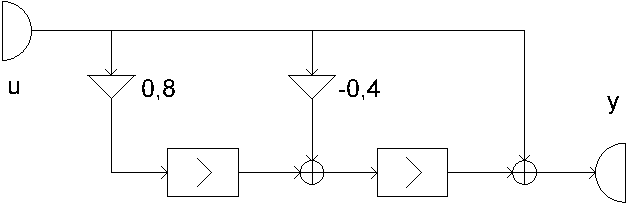
\includegraphics{hf3-kapcs.ps}
\end{center}

\end{document}
